
\section{Mehrdimensionale Integralrechnung}

\subsection{Lebesgue Maß}

Für offene Intervalle $(a_i,b_i) \subset \mathbb{R}$ mit $a_i \leq b_i$ nennen wir $I := (a_1,b_1) \times \cdots \times (a_n,b_n)$ einen $n$-dimensionalen Quader 
und $\bar{I}:= [a_1, b_1] \times \cdots \times [a_n,b_n]$ seinen Abschluss. Wir definieren das Volumen 
\begin{align*}
\text{vol} (I):=   \prod_{i = 1}^n (b_i -a_i)  \; .
\end{align*}

Mit 
$$\mathbb{I}(n): = \{   (a_1,b_1) \times \cdots \times (a_n,b_n) \; | \;  (a_i, b_i) \subset \mathbb{R} \}$$
 bezeichnen wir die Menge aller $n$-dimensionalen Quader und mit
$$\mathbb{I}^0(n): = \{   (a_1,b_1) \times \cdots \times (a_n,b_n) \; | \;  (a_i, b_i) \subset \mathbb{R}  \text { und } a_k = b_k \text{ für ein k}\}$$ 
die Menge der degenerierten Quader.   Für eine Menge $A \subset \mathbb{R}^n$ bezeichnen wir eine Menge von Quadern 
$$ \biggl \{ I_j \; | \;  I_j \in \mathbb{I}(n)   \text{ mit } A \subset \bigcup_j I_j  \biggr \}$$ als Hüllquader für $A$.
\begin{Definition}[Lebesguesche äußere Maß]
Für eine Menge $A \subset \mathbb{R}^n$ definieren wir das Lebesguesche äußere Maß durch 
\begin{align*}
\mu (A):=   \inf \biggl \{ \sum_{j=1}^{\infty}   \text{vol} (I_j)\; ; \; I_j \in \mathbb{I}(n); A \subset \bigcup_{j= 1}^{\infty} I_j \biggr \} 
\end{align*}
Falls für alle Hüllquader $\text{vol} (I_j) = \infty$ gilt, so setzen wir $\mu (A) = \infty$.
\end{Definition}

\begin{Definition}[Erinnerung Infimum]
\end{Definition}

\begin{Definition}[Nullmenge]
Eine Menge $N \subset \mathbb{R}^n$ mit $\mu (N) = 0$ heißt Nullmenge.
\end{Definition}


\begin{Bemerkung}
\label{massmonton}
Für $A \subset B \subset \mathbb{R}^n$ ist $\mu(A) \leq \mu(B)$
\end{Bemerkung}
\begin{proof}
Da $A \subset B$ Teilmenge ist, sind Hüllquader von $B$  auch Hüllquader von $A$ und damit  $\mu(A) \leq \mu(B)$.
\end{proof}

\begin{Satz}[$\sigma$-subadditivität]
Sei $A_j \subset \mathbb{R}^n$ eine Folge von Mengen. Dann gilt
\begin{align*}
\mu (\bigcup_j^{\infty} A_j ) \leq \sum_{j=1}^{\infty} \mu(A_j)
\end{align*}
\end{Satz}
\begin{proof}
Für jedes $A_j$ und $\epsilon > 0$ können wir  eine geeignete Überdeckung  $A_j \subset \bigcup_k  K_{j,k}$ mit Hüllquadern $K_{j,k}$ finden, so dass 
 $\sum_k \text{vol} (K_{j,k}) \leq \mu(A_j) + \frac{\epsilon}{2^{j+1}}$.
Da $ \bigcup_j A_j \subset \bigcup_j \bigcup_k  K_{j,k}$ eine Überdeckung mit Hüllquadern ist, folgt
\begin{align*}
\mu \biggl (  \bigcup A_j  \biggr) \leq \sum_j \sum_k \text{vol} (K_{j,k}) \leq  \bigl( \sum_j  \mu(A_j) + \frac{\epsilon}{2^{j+1}} \bigr)  = \bigl (\sum_j \mu(A_j) \bigr ) + \epsilon
\end{align*}
(Die letzte Gleichung beruht auf dem Wert der \href{https://de.wikipedia.org/wiki/Geometrische_Reihe}{geometrischen Reihe}).
Da die letzte Aussage für beliebiges $\epsilon > 0$ gilt, folgt die Behauptung.
\end{proof}


\begin{Bemerkung}
\label{volimu}
Für $I \in \mathbb{I}(n)$ gilt $\mu(I) = \text{vol}(I)$.
\end{Bemerkung}
\begin{proof}
Seien  $I_j \in \mathbb{I}(n)$ mit $I \subset \bigcup_j  I_j$. Da $I$ beschränkt und abgeschlossen ist, ist $I$ kompakt. Damit reichen endlich 
viele Intervalle, um $I  \subset  \bigcup_{j=1}^n  I_j$ zu überdecken. Für endlich viele Intervalle ist es einfach zu zeigen, dass
$$\text{vol} (I) \leq \sum_{j=1}^n \text{vol} (I_j) $$
gilt. Damit folgt die Behauptung.
\end{proof}

\begin{Satz}
Für $I \in \mathbb{I}(n)$  und $A \subset \mathbb{R}^n$ mit $I \subset A \subset \bar{I}$ gilt $\mu (A) = \text{vol}(I)$.
\end{Satz}
\begin{proof}
Mit $I_0:=  I$ und $I_j := \emptyset$ ist $I \subset \bigcup_j I_j$ und damit gilt 
\begin{align*}
\mu(I) \leq \sum_j \text{vol}(I_j) = \text{vol}(I)
\end{align*}

Es sei $\mathcal{A}_0 := \{ A  \in \mathbb{R}^n  \; | \;  I^0 \subset A \subset \bar{I^0}  \text{  mit } I^0 \in \mathbb{I}^0(n) \}$. Für $A_0 \in \mathcal{A}_0$ gibt es 
$\epsilon > 0$ und $I_{\epsilon} \in \mathbb{I}(n)$ mit $A \subset I_{\epsilon}$ und $\text{vol} (I_{\epsilon})  \leq \epsilon$ und damit $\mu(A_0) = 0$.
Zu $I \in \mathbb{I}(n)$ gibt es $2n$-Seiten $J_j \in \mathcal{A}_0$ mit 
$\bar{I} = I \cup \bigcup_{j= 1}^{2n} J_j$. Aus der $\sigma$-subadditivität folgt
\begin{align*}
\mu(\bar{I})  \leq \mu(I) + \sum_{j=1}^{2n} \mu(J_j) = \mu (I)
\end{align*}
 Für $I \subset A \subset \bar{I}$ folgt damit und mit der Monotonie
$$ \mu(I) = \mu(A) = \mu(\bar{I}) \;. $$
Mit Bemerkung \ref{volimu} folgt die Behauptung.

\end{proof}


Es sei $A, D \subset \mathbb{R}^n$  beschränkte Teilmenge mit $A \subset D$.  
Man kann einerseits das Volumen $\mu(A)$, als auch das Volumen 
$\mu_D(A) :=  \mu(D) - \mu(D  \setminus  A)$ berechnen. Man approximiert hierbei das Volumen von $A$ einmal mit Hüllquadern von außen und einmal von innen.
 
\begin{figure}[!tbp]
  \centering
  \begin{minipage}[b]{0.49\textwidth}
    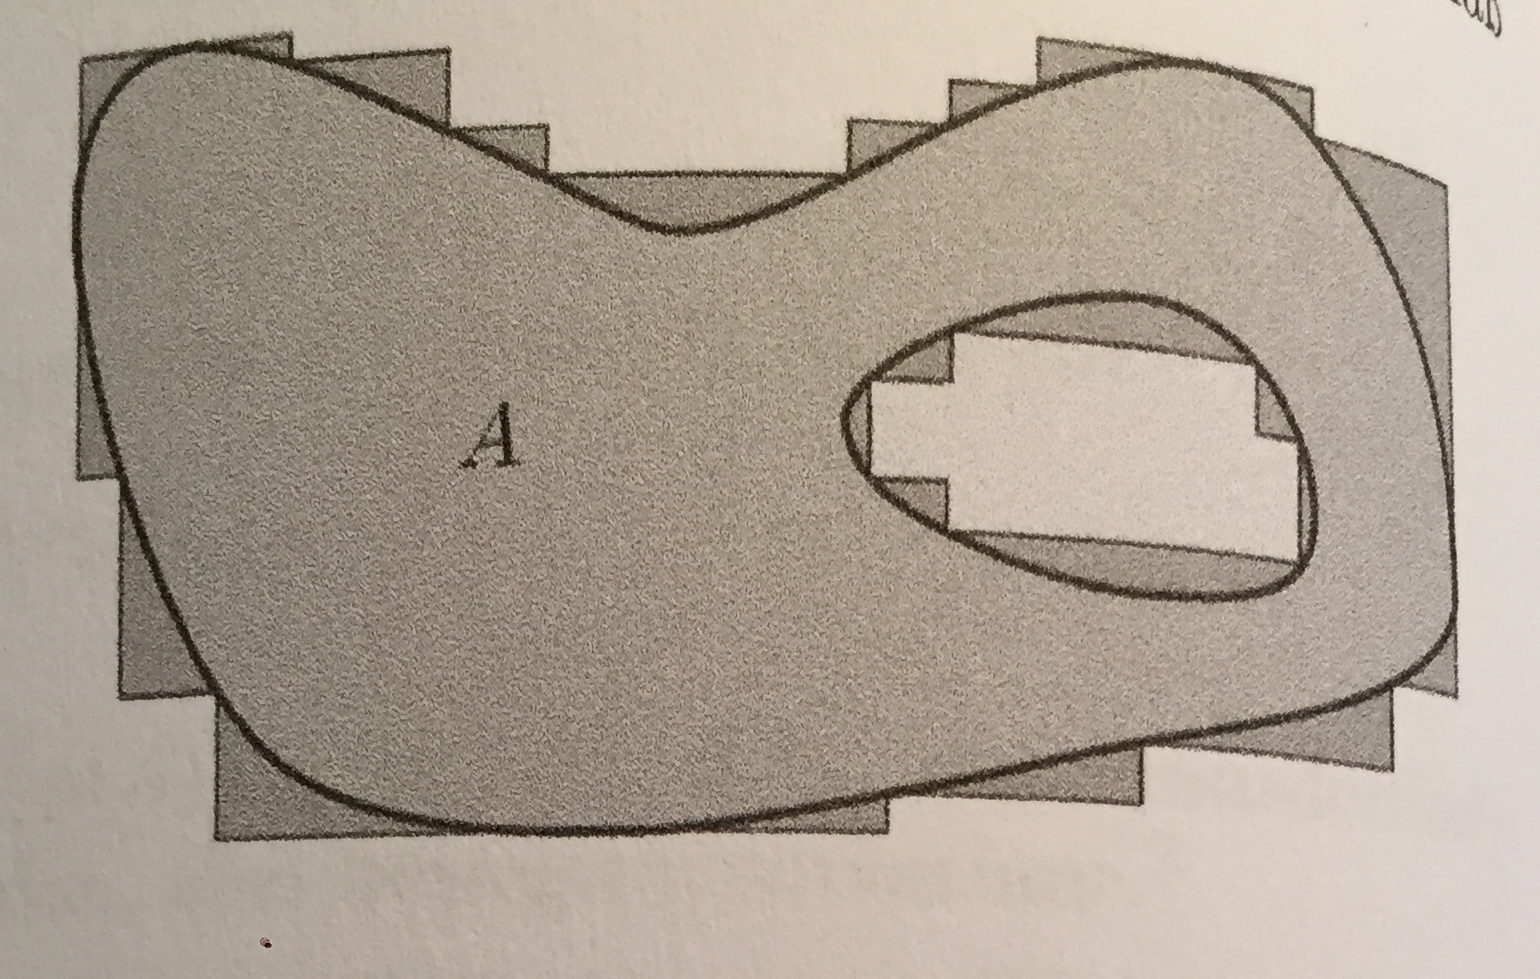
\includegraphics[width=1.0\textwidth]{images/am}
    \caption{Äußeres Maß}
  \end{minipage}
  \hfill
  \begin{minipage}[b]{0.49\textwidth}
    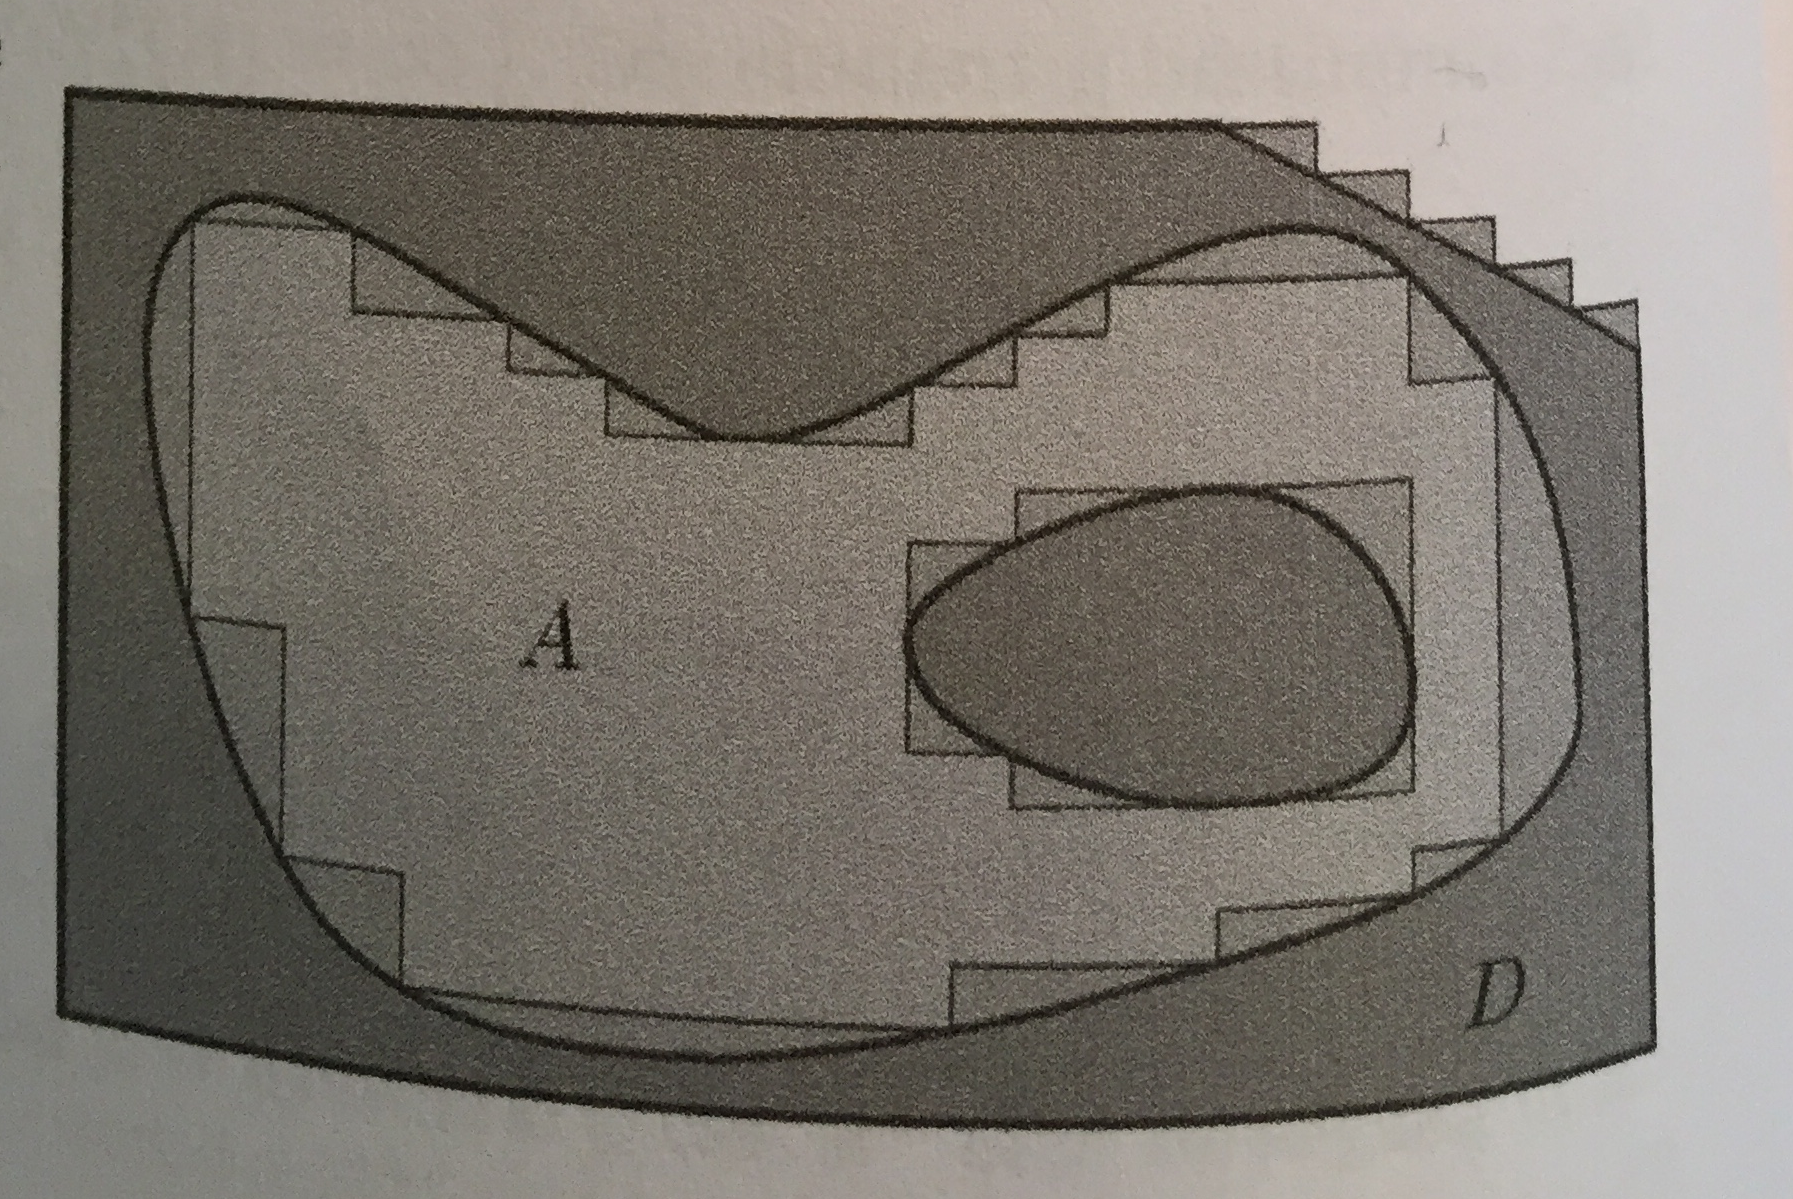
\includegraphics[width=1.0\textwidth]{images/im}
    \caption{Inneres Maß}
  \end{minipage}
\end{figure}

Es ist daher sinnvoll von einer messbaren Menge zu sprechen, wenn diese beiden Volumen übereinstimmen, also
$\mu_D(A) = \mu(A)$ gilt. Dies ist gleichbedeutend mit der Bedingung $\mu(D) = \mu(A) + \mu(D  \setminus A)$. 
Für festes $D$ wären somit alle Mengen $A$ messbar, für die das äußere Lebesgue Maß additiv ist auf der Zerlegung $D = A \cup D \setminus A$. 
Lässt man die Bedingungen der Beschränktheit und $A \subset D$ fallen, gelangt man zu folgender Definition.

\begin{Definition}[$\mu$-messbare Menge]
Eine Menge $A \subset \mathbb{R}^n$ heißt messbar, falls für alle $D \subset  \mathbb{R}^n$ gilt
\begin{align*}
\mu(D) =  \mu(A \cap D) + \mu(A^c \cap D)
\end{align*}
Da wir die $\sigma$-subadditivität bereits nachgewiesen haben, können wir diese Bedingung auf
\begin{align*}
\mu(D) \geq  \mu(A \cap D) + \mu(A^c \cap D)
\end{align*}
reduzieren. Die Menge aller messbaren Mengen bezeichnen wir mit $\mathcal{A}$.
\end{Definition}

\begin{Bemerkung}
Nullmengen sind messbar.
\end{Bemerkung}
\begin{proof}
Es sei $N, D \subset \mathbb{R}^n$ mit $\mu(N)= 0$. Wegen der Monotonie von $\mu$ ist $0 \leq \mu (N \cap D) \leq \mu(N) = 0$ und somit ist $N \cap D$ auch eine Nullmenge. Wir erhalten damit und nochmaliger Monotonie von $\mu$
$$ \mu(N \cap D) + \mu (N^c \cap D) =  \mu (N^c \cap D) \leq \mu(D) $$
und damit ist $N$ messbar.
\end{proof}



\subsubsection*{$\sigma$-Algebra der messbaren Mengen}
Die Menge der messbaren Mengen $\mathcal{A}$ hat einige besondere Eigenschaften. Wir geben hier nur diese Eigenschaften ohne Beweis an. Die Beweise verwenden im wesentlichen Techniken, die wir bereits kennengelernt haben.
\begin{itemize}
\item Für eine Folge $A_i \in \mathcal{A}$ von messbaren Mengen mit $A_i \cap A_j  =  \emptyset$ ist $\mu (\bigcup_i A_i ) = \sum_i \mu(A_i)$.
\item Ist $A \in \mathcal{A} $, so ist auch $A^c \in \mathcal{A} $.
\item Für eine Folge $A_i \in \mathcal{A}$ messbarer Mengen  ist $\bigcup_i A_i \in \mathcal{A}$ messbar.
\end{itemize}



\begin{Satz}[Charakterisierung messbarer Mengen]
Eine Menge $A$ ist genau dann messbar, wenn $A = S \cup N$, wobei $N$ eine Nullmenge und $S$ Vereinigung von kompakten Mengen ist.
\end{Satz}


\subsection{Lebesgue Integral}

\begin{Definition}
Für eine Teilmenge $A \subset \mathbb{R}^n$ heißt
$$ 1_A (x): = \begin{cases} 1 \text{  falls }   x \in A  \\  0  \text{  sonst}  \end{cases}$$
Indikatorfunktion.
\end{Definition}

\begin{Definition}
Eine Funktion 
$$ \varphi(x) := \sum_{k=1}^m c_k 1_{I_k}$$ mit $c_k \in \mathbb{R}$ und $I_k \in \mathbb{I}(n)$ mit $I_l \cap I_h = \emptyset$ für $i \neq j$
heißt Treppenfunktion.
\end{Definition}

\begin{figure}[H]
      \centering
    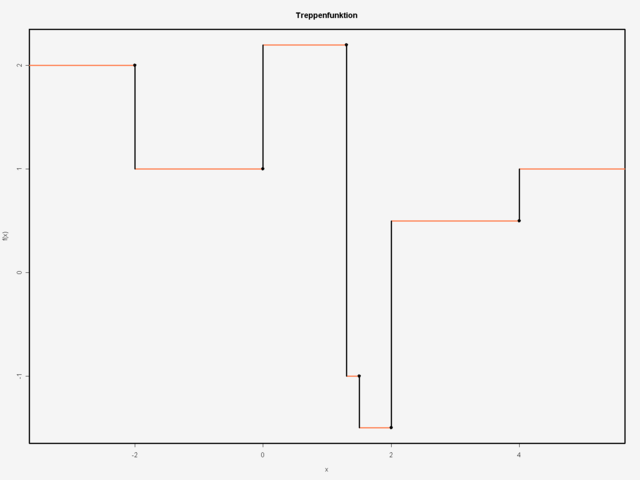
\includegraphics[width=0.8\textwidth]{images/640px-Stepfunction1}
      \caption{Quelle: Wikipedia: https://commons.wikimedia.org/wiki/File:Stepfunction1.png}

\end{figure}



\begin{Bemerkung}
Seien $\varphi(x) =   \sum_{k=1}^m  c_k 1_{I_k}$ und $\psi(x) =  \sum_{j=1}^l  u_j 1_{I_j}$. Dann definiert
$(\varphi + \psi)(x) := \sum_{k=1}^m \sum_{j=1}^l   (c_k + u_j) 1_{I_{k,j}}$ mit $I_{k,j}:= I_k \cap I_j$ eine Treppenfunktion (nach entsprechender Umnummerierung zu einem einzigen Summenzeichen).
\end{Bemerkung}


\begin{Definition}
Für eine Treppenfunktion $ \varphi(x) := \sum_{k=1}^m c_k 1_{I_k}$ definieren wir das Integral durch
$$\int_{\mathbb{R}^n} \varphi d\mu := \sum_{k =1}^m  c_k \mu(I_k) \; . $$
\end{Definition}

\begin{Satz}
\label{TFB}
Seien $\varphi(x) =   \sum_{k=1}^m  c_k 1_{I_k}$ und $\psi(x) =  \sum_{j=1}^l  u_j 1_{I_j}$ zwei Treppenfunktionen.
Für das Integral von Treppenfunktion gilt:
\begin{itemize}
\item Ist $\varphi(x) = \psi(x)$ für alle $x$, dann ist $\int_{\mathbb{R}^n} \varphi d\mu = \int_{\mathbb{R}^n} \psi d\mu$ (Das integral hängt nicht von der Zerlegung der Treppenfunktion ab und  ist wohldefiniert)
\item $\int_{\mathbb{R}^n} \alpha \varphi  + \beta \psi d\mu = \alpha \int_{\mathbb{R}^n}  \varphi d\mu + \beta  \int_{\mathbb{R}^n}  \psi d\mu$
\item $ \biggl|  \int_{\mathbb{R}^n} \varphi d\mu  \biggr| \leq \int_{\mathbb{R}^n} | \varphi | d\mu$
\item Ist $\varphi(x) \leq \psi(x)$ für alle $x$, so ist $\int_{\mathbb{R}^n} \varphi d\mu \leq \int_{\mathbb{R}^n} \psi d\mu$ 
\end{itemize}
\end{Satz}

\begin{proof}
Der Beweis wird über eine vollständige Induktion geführt. Der Induktionsanfang ist einfach zu zeigen. 
Wir nehmen an, die Aussage gilt für alle Dimensionen $k < n$.
Zerlege $\mathbb{R}^n = \mathbb{R}^p \times \mathbb{R}^{n-p}$. Jeder Quader $I \in \mathbb{I}(n)$ zerlegt sich damit ebenfalls in ein Produkt 
$I = I' \times I''$ mit $I'  \in \mathbb{I}(p)$ und  $I''  \in \mathbb{I}(n-p)$ und für $z = (x,y) \in  \mathbb{R}^p \times \mathbb{R}^{n-p}$ gilt $1_{I} (z) = 1_{I'}(x) \cdot 1_{I''}(y)$. Es sei nun $\varphi(z):=   \sum_{k=1}^m  c_k 1_{I_k}(z)$ eine Treppenfunktion auf $ \mathbb{R}^p \times \mathbb{R}^{n-p}$. Für jedes $y \in \mathbb{R}^{n-p}$ definiert  $\varphi_y(x)=   \sum_{k=1}^m  c_k 1_{I''_k}(y) \cdot 1_{I'_k}(x)$ eine Treppenfunktion auf $\mathbb{R}^{n-p}$. 
Nach Induktionsvoraussetzung hängt das Integral 
$$\int_{\mathbb{R}^p}  \varphi_y(x) d \mu' = \sum_{k=1}^m  c_k \mu'(I'_k)  \cdot 1_{I''_k}(y)  =: \phi(y)$$
nicht von der Zerlegung der Treppenfunktion ab. $\phi(y)$ ist wiederum eine Treppenfunktion auf $\mathbb{R}^{n-p}$ und Nach Induktionsvoraussetzung hängt das Integral 
$$\int_{\mathbb{R}^{n-p}}  \phi(y) d \mu'' = \sum_{k=1}^m  c_k \mu'(I'_k)  \cdot \mu'' (I''_k)(y) $$
nicht von der Zerlegung der Treppenfunktion ab. Somit gilt
$$\int_{\mathbb{R}^{n-p}} \int_{\mathbb{R}^p}  \varphi_y(x) d \mu'  d \mu''  =   \sum_{k=1}^m  c_k \mu'(I'_k)  \cdot \mu''(I''_k)(y) = \sum_{k=1}^m  c_k  \mu(I_k)  = \int_{\mathbb{R}^n} \varphi(z) d\mu\;.$$
Die linke Seite hängt  damit nicht von der Zerlegung der Treppenfunktion ab und alle Behauptungen können so auf den Fall $n=1$ zurückgeführt werden.
\end{proof}

\begin{Bemerkung}[Satz von Fubini für Treppenfunktionen]
\label{FTF}
Es gilt $$\int_{\mathbb{R}^n} \varphi(x,y) d \mu = \int_{\mathbb{R}^{n-p}} \biggl (\int_{\mathbb{R}^{p}}  \varphi(x,y) d \mu' \biggr ) d \mu''$$
\end{Bemerkung}
\begin{proof}
Siehe Beweis des letzten Satzes.
\end{proof}


\subsubsection{Die $L^1$-Halbnorm}
Der Fall $\infty$ ist bei den folgenden Betrachtungen immer als möglicher Fall zu berücksichtigen.

\begin{Definition}
Eine Hüllreihe zu einer Funktion $f :\mathbb{R}^n \to \mathbb{R}$ ist eine Reihe $\phi(x):= \sum_{k=1}^{\infty} c_k  1_{I_k} (x)$ mit den folgenden Eigenschaften:
\begin{itemize}
\item $c_k \in \mathbb{R}$ sind positive reelle Zahlen $c_k >0$.
\item $I_k \subset \mathbb{R}^n$ sind offene Quader.
\item Für alle $x \in \mathbb{R}^n$ gilt $|f(x) | \leq \phi(x)$.
\end{itemize}
\end{Definition}


\begin{Definition}
Der Innhalt einer Hüllreihe $\phi(x):= \sum_{k=1}^{\infty} c_k  1_{I_k} (x)$ ist definiert durch 
$$I (\phi) := \sum_{k=1}^{\infty} c_k \;  \mu(I_k) \; .$$
\end{Definition}


\begin{Definition}
Die $L^1$-Halbnorm einer Funktion $f :\mathbb{R}^n \to \mathbb{R}$ is definiert durch das Infimum der Inhalte der Hüllreihen zu $f$
$$ || f ||_1 : = \inf  \biggl \{   I(\phi) \; | \; \phi  \text{ ist Hüllreihe zu  }  f \biggr \} \; .$$
\end{Definition}

\begin{Lemma}[Verallgemeinerte Dreiecksungleichung]
\label{vdug} 
Für nicht negative Funktionen $f_k  :\mathbb{R}^n \to \mathbb{R}_{\geq 0}$ gilt
$$ \biggl | \biggl | \sum_{k=1}^{\infty} f_k \biggr | \biggr |_1 \leq  \sum_{k=1}^{\infty} || f_k  ||_1 \; .$$
\end{Lemma}

\begin{proof}
Zu $\epsilon > 0$ und $f_k$ wählen wir eine Hüllreihe $\phi_k = \sum_{i} c_{ik} 1_{I_{ik}}$ mit Inhalt
$$ I(\phi_k) =  \sum_{i} c_{ik} \; \mu (1_{I_{ik}}) = || f_k||_1 + \frac{\epsilon}{2^k} \;.$$ Dann ist $\phi := \sum_{k,i} c_{ik} 1_{I_{ik}}$ eine Hüllreihe der Funktion $\sum_k f_k$ mit 
$$ I(\phi) = \sum_{k,i} c_{ik}  \; \mu (I_{ik}) = \sum_k \biggl( \sum_i  c_{ik} \; \mu (I_{ik})\biggr) \leq \sum_k || f_k ||_1 + \epsilon$$
Mit  $ \bigl | \bigl | \sum_{k=1}^{\infty} f_k \bigr | \bigr |_1 \leq I(\phi) $ und $\epsilon \to 0$ folgt die Behauptung.
\end{proof}

\begin{Bemerkung}[Rechenregeln]
Für $f,g : \mathbb{R}^n \to \mathbb{R}$ und $c \in \mathbb{R}$ gilt:
 \begin{itemize}
\item $|| cf ||_1 \leq |c| || f ||_1$. 
\item $|| f +g ||_1 \leq  ||f ||_1 + ||g||_1$
\item Aus $|| f (x)||_1 \leq g(x)$ für alle $x$ folgt $|| f ||_1 \leq || g ||_1$.
\end{itemize}
\end{Bemerkung}
\begin{proof}

 \begin{itemize}
\item Für eine Hüllreihe $\varphi$ von $f$ ist $|c| \cdot \varphi$ eine Hüllreihe von $c \cdot f$. 
\item  Da $|f +g | \leq | f | + | g |$ folgt Behauptung aus (iii) und der verallgemeinerten Dreiecksungleichung.
\item Hullreihen sind immer größer-gleich der Funktion und damit haben größere Funktionen größere Hüllreihen.
\end{itemize}
\end{proof}

\begin{Lemma}[Fundamentallemma]
Für die charakteristische Funktion $1_{I}$ eines Quaders $I$ gilt 
$$ || 1_I ||_1 = \mu(I) =  \text{vol} (I) = \int 1_I d \mu$$
\end{Lemma}
\begin{proof}
$ 1 \cdot 1_I$ ist eine Hüllfunktion von $1_i$ und damit gilt $|| 1_I || \leq \mu(I)$. 
Sei $\phi(x) = \sum_k c_k 1_{I_k} $ eine Hüllreihe von $1_i$ und $\epsilon >0$. Da $\phi(x) \geq 1$ gibt es für jedes $x$ einen Index $N(x)$ mit 
$\sum_{k=1}^{N(x)} c_k 1_{I_k} \geq 1 - \epsilon$. Da die $I_k$ offen sind, gibt es für jedes $x$ eine Umgebung $U(x)$, so dass letztere Gleichung gilt. Da $\bar{I}$ kompakt ist (beschränkt und abgeschlossen), überdecken endlich viele $U(x_1), \cdots , U(x_n)$ den Quader $I$. Mit $N:= \max \{ N(x_1), \cdots , N(x_n)$ folgt $\sum_{k=1}^N c_k 1_{I_k} \geq (1-\epsilon) 1_I$. Aus Satz \ref{TFB} (iii) folgt
$$ I (\phi) = \sum_k c_k \mu(I_k) \geq \sum_{k=1}^N c_k \mu (I_k) \geq (1 - \epsilon) \mu(I) \;.$$
Mit $\epsilon \to 0$ folgt $I (\phi) \geq \mu(i)$ und damit insgesamt die Behauptung.  
\end{proof}


\begin{Lemma}
\label{normbetragintegral}
Für jede Treppenfunktion $\varphi$ auf $\mathbb{R}^n$ gilt
$$ || \varphi ||_1 = \int | \varphi | d \mu  \; .$$
\end{Lemma}


\subsubsection{Integration über den $\mathbb{R}^n$}

\begin{Definition}
Eine Funktion $f : \mathbb{R}^n \to \mathbb{R}$ heißt integrierbar, falls eine Folge von Treppenfunktionen  $\varphi_k$ existiert mit
$$ || f -  \varphi_k ||_1 \to 0 \text{ für } k \to \infty \;. $$
In diesem Fall heißt
$$ \int_{\mathbb{R}^n} f(x) d \mu := \lim_{k \to \infty}  \int_{\mathbb{R}^n}  \varphi_k d \mu$$
das Integral von $f$ über $\mathbb{R}^n$.
\end{Definition}

\begin{Bemerkung}
\hfill
\begin{itemize}
\item Die reelle Zahlenfolge $\int \varphi_k d\mu$ ist eine Cauchyfolge und damit konvergent. 
\item Der Grenzwert ist unabhängig von der Folge $\varphi_k$.
\end{itemize}

\end{Bemerkung}
\begin{proof}
Für Treppenfunktionen $\psi$ und $\xi$ gilt 
\begin{align*}
\biggl | \int \psi d \mu - \int \xi d \mu \biggr |  &  \leq \int | \psi - \xi | d \mu = || \psi - \xi ||_1 \\
& \leq  || \psi - f ||_1 +  || f - \xi ||_1
\end{align*}
woraus die Behauptungen folgen.
\end{proof}

\begin{Satz}
\label{ibf}
Ist $f$ über $\mathbb{R}^n$ integrierbar, so auch $|f|$ und es gilt
$$ \biggl | \int f d \mu \biggr | \leq \int  | f | d \mu = || f ||_1 \; .$$
\end{Satz}
\begin{proof}
Sei $f$ integrierbar und $\varphi_k$ eine Folge von Treppenfunktionen mit $|| f - \varphi_k ||_1 \to 0$. 
Aus $\bigl | | f | - | \varphi_k | \bigr | \leq | f -\varphi | $ ergibt sich wegen der Monotonie der $L^1$-Norm
$$\bigl |  \bigl |  | f | - | \varphi_k | \bigr | \bigr |_1 \leq \bigl |  \bigl |   f  -  \varphi_k  \bigr | \bigr |_1  \; .$$ 
Damit gilt $\bigl |  \bigl |  | f | - | \varphi_k | \bigr | \bigr |_1 \to 0$ und somit ist $|f|$ integrierbar und mit der Abschätzung von Beträgen für Treppenfunktionen aus Satz \ref{TFB} gilt 
\begin{align*}
\biggl | \int f d \mu \biggr | = \biggl | \lim_k \int \varphi_k d \mu \biggr | \leq  \int |\varphi_k| d \mu = \int |f| d\mu
\end{align*} 
und damit der erste Teil der Behauptung. 
Mit der Dreiecksungleichung erhalten wir
$$ || f || - ||  f - \varphi ||_1 \leq || \varphi_k ||_1  \leq || f ||_1 + || f - \varphi_k ||_1 $$
und wegen $|| \varphi_k ||_1 = \int | \varphi_k | d \mu \to \int | f | d \mu$ folgt die Behauptung.
\end{proof}


\begin{Bemerkung}[Rechenregeln]
Sind $f$ und $g$ integrierbar, so gilt
\begin{itemize}
\item $ \alpha f + \beta g$ mit $\alpha, \beta \in \mathbb{R}$ ist integrierbar mit 
$$\int \alpha f + \beta g d\mu = \alpha \int f d\mu + \beta \int g d \mu \; .$$ 
\item Aus $f(x) \leq g(x)$ für alle $x \in \mathbb{R}^n$ folgt $\int f d \mu \leq \int g d \mu$.
\item Ist $g$ zusätzlich beschränkt, so ist auch $f \cdot g$ integrierbar.
\end{itemize}
\end{Bemerkung}
\begin{proof}
\begin{itemize}
\item Sind $\phi_k$ und $\psi_k$ approximierende Folge von  Treppenfunktionen von $f$ und $g$, so ist $\alpha \phi_k + \beta \psi_k$ eine approximierende Folge von $\alpha f + \beta g$.
\item Nach Satz \ref{ibf} ist $\int (g-f) d \mu = || g - f ||_1 \geq 0$.
\end{itemize}
\end{proof}


\begin{Bemerkung}
Ist $f$ integrierbar, so auch $f^+ := \max(f,0)$ und $f^- := \min(f,0)$. Damit ist $f = f^+ + f^-$ genau dann integrierbar, wenn $f^+$ und $f^-$ integrierbar sind. Da $- f^- \geq 0$ ist, kann man sich in Beweisen häufig auf den Fall $f \geq 0$ beschränken.
\end{Bemerkung}
\begin{proof}
Es ist $ \max(f,0) = \frac{1}{2} (f + | f |)$ und  $ \min(f,0) = \frac{1}{2} (f - | f |)$ und die Behauptung folgt aus den Rechenregeln.
\end{proof}

\begin{Definition}[Integration über Teilmengen]
Für  eine Teilmenge $A \subset \mathbb{R}^n$ und eine Funktion $f: A \to \mathbb{R}$ heißt
$$  f_A (x) : = \begin{cases}  f(x) \text{ für } x \in A \\ 0  \text{ für } x \in \mathbb{R}^n \setminus A \end{cases}$$ 
die triviale Fortsetzung von $f$ auf $\mathbb{R}^n$. $f$ heißt integrierbar über $A$, falls $f_A$ über $\mathbb{R}^n$ integrierbar ist und in diesem Fall bezeichnen wir mit $$ \int_A f(x) d \mu := \int f_A (x) d\mu$$ als das Integral von $f$ über $A$.
\end{Definition}




\begin{Satz}[Kleiner Satz von B. Levi]
\label{KBL}
Zu $f: \mathbb{R}^n \to \mathbb{R}$ gebe es eine monoton wachsende Folge $\varphi_k$ von Treppenfunktionen mit
\begin{itemize}
\item Für alles $x \in \mathbb{R}^n$ git $\lim_{k \to \infty} \varphi(x) =  f(x)$. $f$ ist also die punktweise gebildete Grenzfunktion der $\varphi_k$.
\item Die reelle Folge der Integrale $\int \varphi_k d \mu $ ist beschränkt.
\end{itemize}
Dann ist $f$ integrierbar und es gilt

$$ \int f d \mu = lim_{k \to \infty}  \int \varphi_k d \mu \; .$$
\end{Satz}

\begin{proof}
Aus $f - \varphi_k = \sum_{i=k}^{\infty} (\varphi_{k+1} - \varphi_k)$ folgt mit der verallgemeinerten Dreiecksungleichung Lemma \ref{vdug}  und Lemma \ref{normbetragintegral}
\begin{align*}
|| f - \varphi_k ||_1 \leq \sum_{i=k}^{\infty} \int | \varphi_{i+1} - \varphi_i | d \mu =  \sum_{i=k}^{\infty} \biggl ( \int  \varphi_{i+1}d \mu -  \int \varphi_i  d \mu \biggr ) \; .
\end{align*}
Die Folge $\int \varphi_k$ ist monoton wachsend und beschränkt und damit konvergent. Bezeichnen wir mit $I$ den Grenzwert, so folgt 
$|| f -\varphi_k ||_1 \leq I - \int \varphi_k d \mu $. Also gilt $|| f -\varphi_k ||_1 \to 0$ für $k \to \infty$ und damit ist $f$ integrierbar und mit der Definition des Integrals folgt die Behauptung.
\end{proof}


\begin{Definition}
Eine Menge $U \subset \mathbb{R}^n$ heißt offen, falls für alle $a \in U$ ein Radius $r >0$ existiert, so dass der Ball $B_r(a) : = \{ x \in \mathbb{R}^n \; | \; ||x -a|| \leq r \} \subset U$ in $U$ enthalten ist.
\end{Definition}

\begin{Satz}
\label{fintu}
Sei $U \subset \mathbb{R}^n$ offen und beschränkt und $f : U \to \mathbb{R}$ stetig und beschränkt. Dann ist $f$ über $U$ integrierbar.
\end{Satz}

\begin{proof}
Da $U$ offen ist, kann  man um jeden Punkt $a \in U$ einen Würfel $W_r(a)$ finden, dessen Mittelpunkt $a$  und dessen Kantenlänge $r$ eine rationale Zahl ist. Damit kann man zu Punkten $a_1, \cdots,  a_n$ Würfel wählen, so dass $W_r(a_i) \cap W_r(a_j) = \emptyset$ für $i \neq j$ und mit $m_i := \min \{ f(x)  | x \in W_r(a_i) \} $ Hüllreihen   $\psi_{a_1, \cdots, a_n} := \sum_{i=1}^n m_i 1_{W_r(a_i)} $  konstruieren mit  $\psi \leq f$. Bezeichnen  wir mit $\mathcal{T} :=  \{ \psi_k  \}$ die abzählbare Menge dieser Treppenfunktionen, so ist $f = \sup \{ \psi \; | \; \psi \in \mathcal{T}  \}$ und $\varphi_k : = max \{ \psi_1, \cdots \psi_k  \}$ eine monoton wachsende Treppenfunktion mit $\varphi_k \to f$. Da $U$ beschränkt ist, gibt es eine Quader $I$ mit $U \subset I$ und mit $M : = \max (f)$  ist $\int \varphi_k d \mu \leq M \mu(I)$ beschränkt. Mit dem Satz von B. Levi folgt die Behauptung. 
\end{proof}


\begin{Satz}[Schnittmenge]
Sei $ A \subset \mathbb{R}^n$. Für $ y \in \mathbb{R}^p$ heißt
$$ A_y :=  \biggl \{    x \in \mathbb{R}^{n-p}  \; | \;  (x,y) \in A \biggr \}$$  
Schnittmenge von $A$ zu $y$.
\end{Satz}


\begin{Satz}[Kleiner Satz von Fubuni]
Sei $A \subset \mathbb{R}^n$ eine offene und beschränkte Teilmenge und $f : U \to \mathbb{R}$  eine stetige und beschränkte Funktion.
Dann ist für jedes $ y \in \mathbb{R}^p$ mit $A_y \neq \emptyset$ die Funktion $f_y(x) := f(x,y)$ über $A_y$ und   
$$ F(y) := \begin{cases}   \int_{A_y} f(x,y) d \mu_{p}  , \text{ falls }  A_y \neq \emptyset 
\\ 0 \text{ sonst } \end{cases} $$
über $\mathbb{R}^{p}$ integrierbar und es gilt 
$$ \int_A f(x,y) d \mu_n = \int_{\mathbb{R}^p}  F(y) d \mu_p \; .$$
 Hierfür schreiben wir auch kurz
$$ \int_A f(x,y) d \mu_n  = \int_{\mathbb{R}^{p} }  \biggl ( \int_{A_y} f(x,y)  d\mu_{n-p} \biggr ) d\mu_p$$
\end{Satz}
\begin{proof}
Wie in Beweis zu Satz \label{fintu} sei  $\varphi_k$ eine monoton wachsende Folge von Treppenfunktionen auf $\mathbb{R}^n$ mit $|| f_A - \varphi_k ||_1 \to 0$.
Für jedes $y \in \mathbb{R}^p$ bilden dann die Funktionen $\varphi_k(x)_y := \varphi_k(x,y)$ eine monoton wachsende Folge von Treppenfunktionen auf $\mathbb{R}^{n-p}$, die gegen $f_y(x):= f_A(x,y)$ konvergiert. Die Folge der Integrale $\int_{\mathbb{R}^{n-p}} \varphi_k(x)_y d \mu_{n-p}$ ist beschränkt,  da $A$ beschränkt ist, und daher gibt es eine Quader $I$ mit $U \subset I$ und  mit $M : = \max (f)$  ist $\int \varphi_k d \mu \leq M \mu(I)$ beschränkt. Mit dem kleinen Satz von B. Levi \ref{KBL}
gilt
$$ F(y) := \lim_{k \to \infty} \int_{\mathbb{R}^{n-p}} \varphi_k(x)_y d \mu_{n-p} \; .$$
Die Funktionen 
$$\phi_k (y) := \int_{\mathbb{R}^{n-p}} \varphi_k (x,y) d \mu_{n-p}$$
sind Treppenfunktionen auf $\mathbb{R}^{p}$ und die Folge $\phi_k$ konvergiert monoton wachsend gegen $F$ und die Folge der Integrale 
$\int \phi_k(y) d \mu_{p}$ ist beschränkt, da  mit dem Satz von Fubini für Treppenfunktionen \ref{FTF} und $\varphi_k \leq f_A$  
$$ \int_{\mathbb{R}^{p}} \phi_k(y) d \mu_{p} = \int_{\mathbb{R}^n} \varphi_k(x,y) d\mu_{n} \leq \int_{\mathbb{R}^n} f_A(x,y) d \mu_{n} \; .$$
Mit dem kleinen Satz von B. Levi ist $F$ integrierbar und es gilt
\begin{align*}
 \int_{\mathbb{R}^{p}}   F(y) d \mu_{p} & = \lim_{k \to \infty}  \int_{\mathbb{R}^{p}}  \phi_k (y) d \mu_{p} =  \lim_{k \to \infty}  \int_{\mathbb{R}^{n}}  \varphi_k(x,y) d \mu_{n} \\
& =   \int_{\mathbb{R}^{n}}  f_A (x,y) d \mu_{n}  \; .
\end{align*} 
\end{proof}


\begin{Satz}[Lebesgue vs. Riemann]
Eine \href{https://de.wikipedia.org/wiki/Regelfunktion}{Regelfunktion} $f$ auf $[a,b] \subset \mathbb{R}$ ist über $[a,b] $ Lebesgueintegrierbar und es gilt 
\begin{align*}
\int_{[a,b]} f(x) d \mu_1 = \int_a^b f(x) dx \; .
\end{align*}
\end{Satz}
\begin{proof}
Sei $\varphi_k$ eine Folge von Treppenfunktionen mit $|| f -\varphi_k ||_{\infty} \to 0$. Da für jede Funktion $h$ auf $[a,b]$ die Abschätzung
$|h| \leq || h ||_{\infty} 1_{[a,b]}$ gilt, folgt auch $$|| f_A -\varphi_{k,A} ||_{1} \to 0$$ und damit ist $f_{[a,b]}$ auch Lebesgueintegrierbar über $[a,b]$ mit Lebesgueintegral
\begin{align*}
\int_{[a,b]} f(x) d \mu= \int_{\mathbb{R}} f_A(x) d\mu = \lim_k \varphi_{k,A} d \mu = \lim_k \int_a^b \varphi_k dx = \int_a^b f (x) dx
\end{align*}
 
\end{proof}

\begin{Beispiel} [Integration über Kreis]
Sei $K := B^2_1(0) := \{   (x,y) \in \mathbb{R}^2 \; | \; \sqrt{x^2 + y^2 } \leq 1\}$. Mit dem kleinen Satz von Fubini erhalten wir
\begin{align*}
\int_K 1 d \mu = &  \int_{-1}^{1} \biggl ( \int_{-\sqrt{1- y^2}}^{\sqrt{1- y^2}} 1 dx \biggr ) dy = \\ 
& =  2 \int_{-1}^{1}  \sqrt{1 - y^2}   \; dy  \\ 
 & (substitution \;   y = sin(u)) =   2 \int_{-\frac{\pi}{2}}^{\frac{\pi}{2}}   \cos(u)^2   \; du = 2 \cdot \frac{\pi}{2} = \pi
\end{align*}
\end{Beispiel}
\begin{figure}[H]
      \centering
    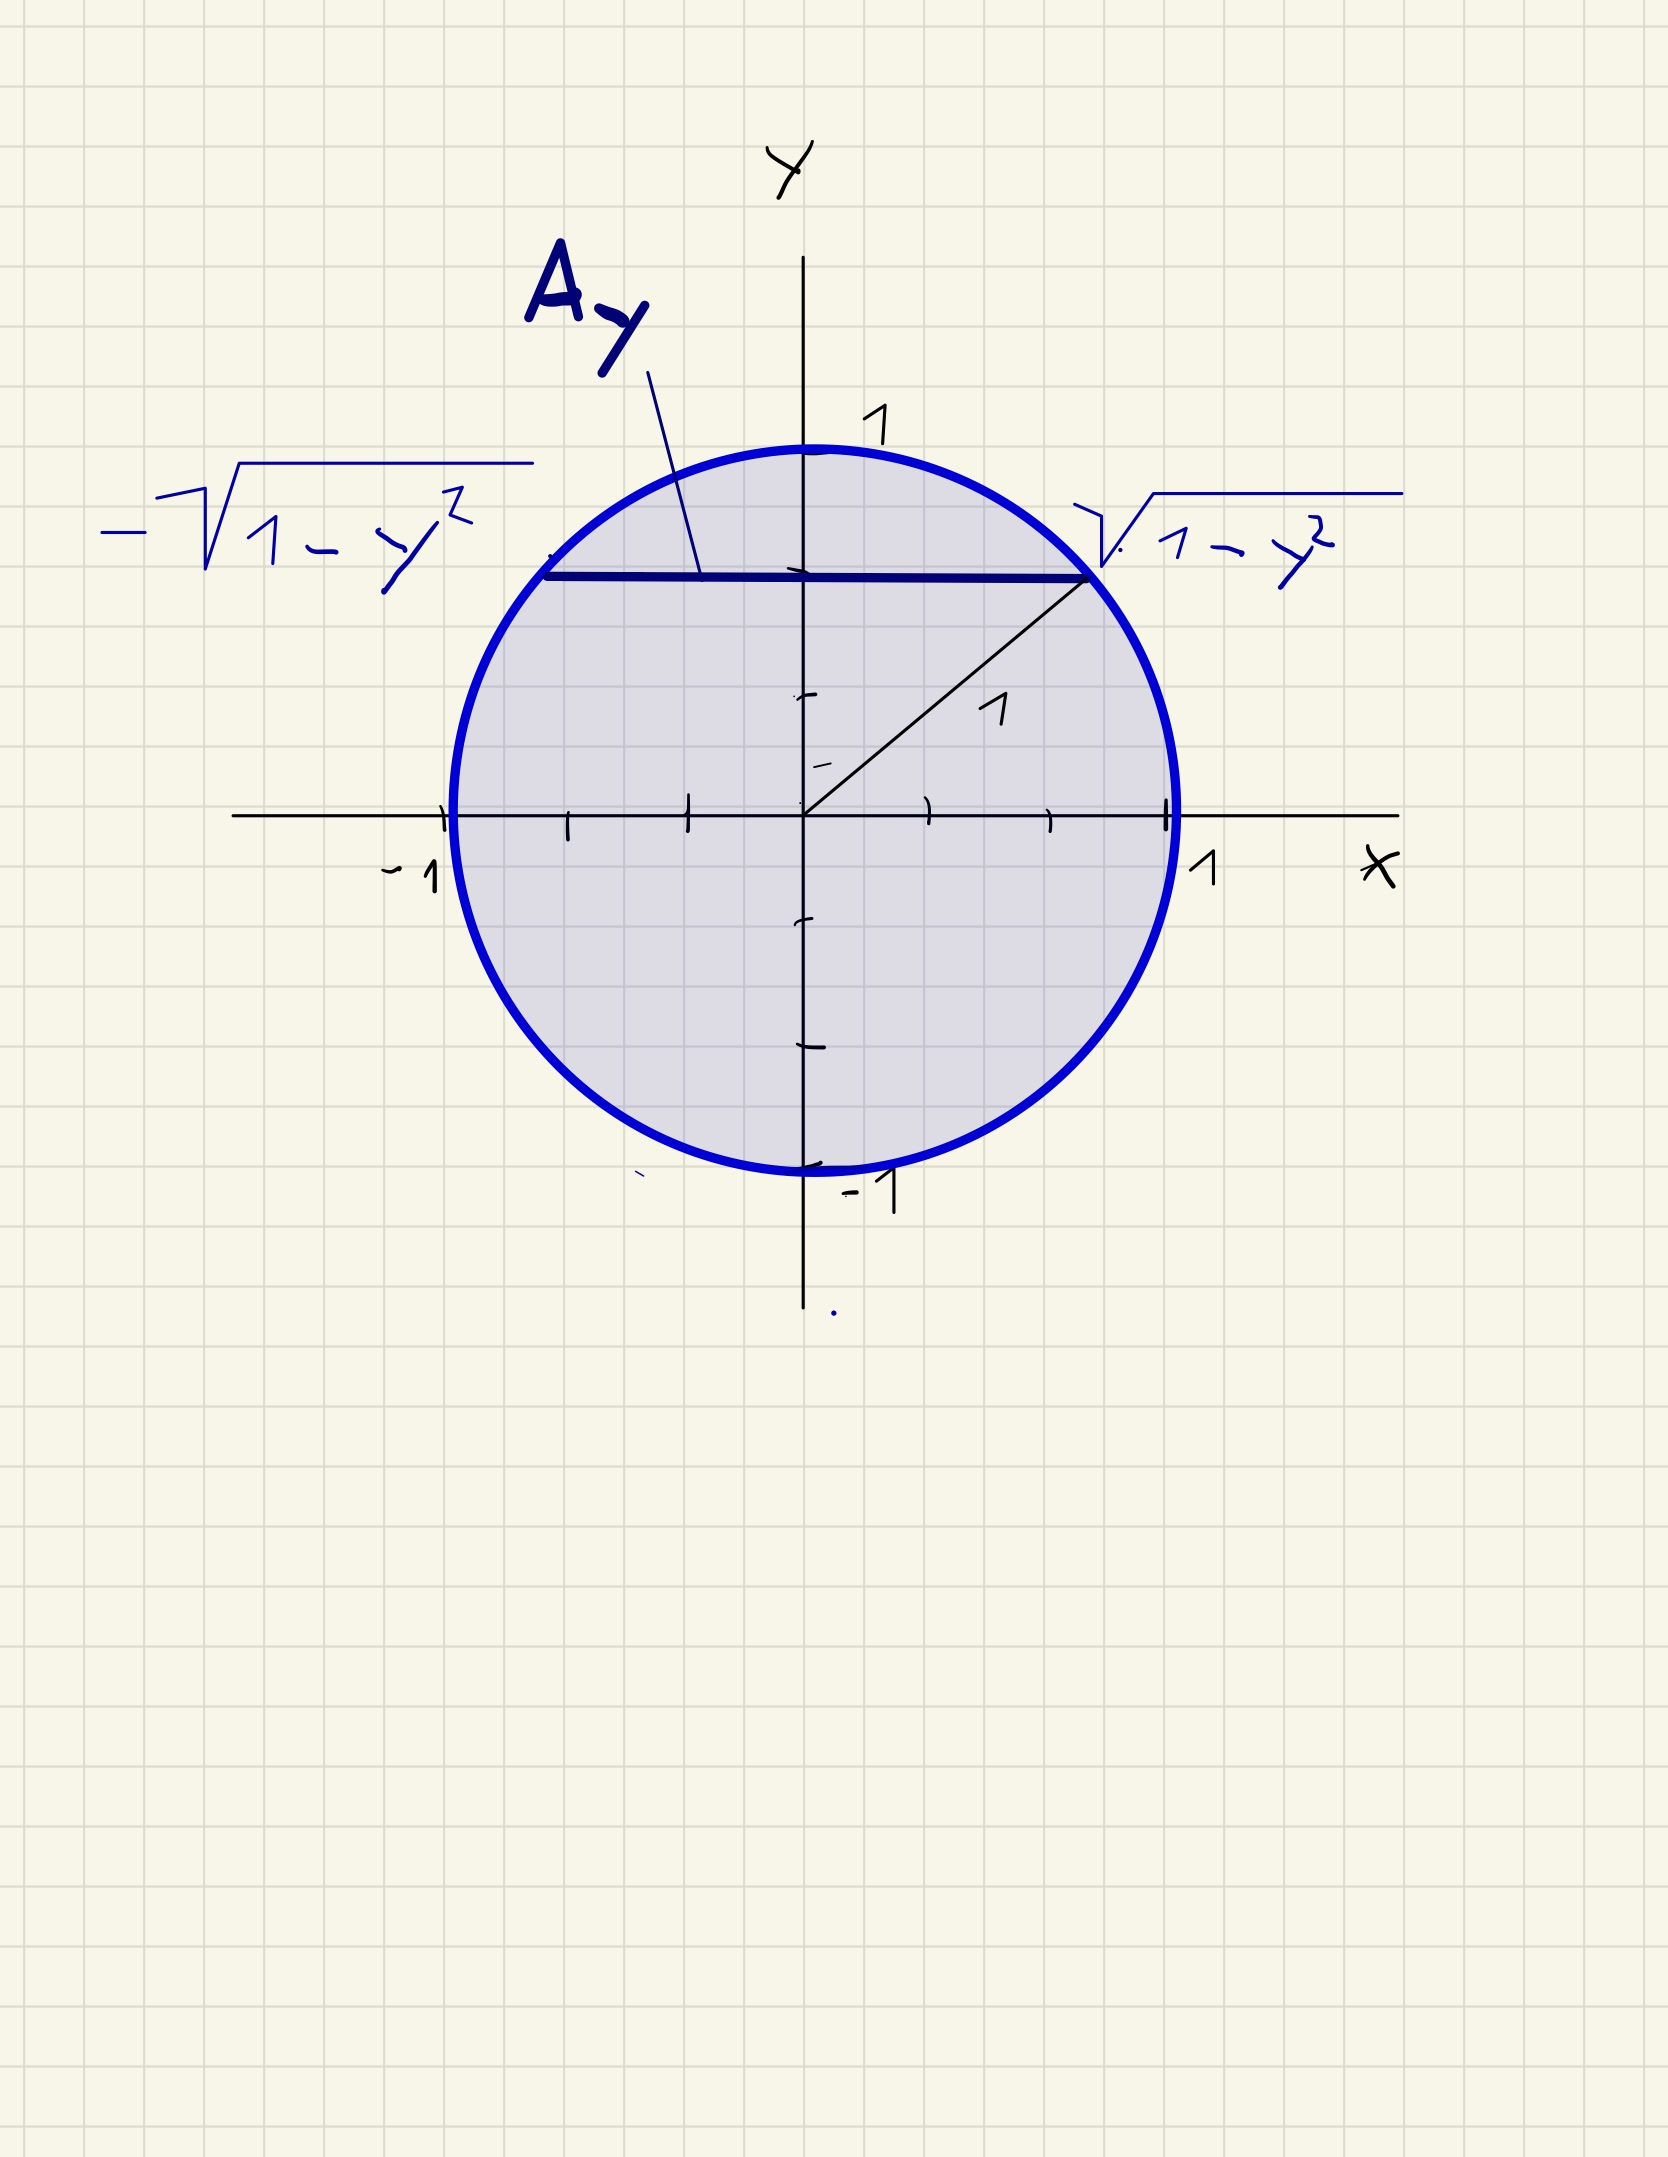
\includegraphics[width=0.8\textwidth]{images/Kreis}
\end{figure}




\begin{Satz}[Produktsatz]
Für Funktionen $f : \mathbb{R}^n \to \mathbb{R}$ und $g: \mathbb{R}^m \to \mathbb{R}$ definiert $(f \otimes g) (x,y) := f(x) \cdot g(x)$ eine Abbildung $f \otimes g : \mathbb{R}^{n+m} \to \mathbb{R}$. Sind $f$  und $g$ integrierbar, so ist $f \otimes g$ integrierbar und es gilt
$$ \int_{\mathbb{R}^{n+m} } (f \otimes g) (x,y) d \mu_{n+m} =  \biggl (    \int_{\mathbb{R}^{n} } f (x) d \mu_{n}  \biggr ) \cdot \biggl (    \int_{\mathbb{R}^{m} } g (y) d \mu_{m}  \biggr )$$
\end{Satz}

\begin{proof}
Für Treppenfunktionen folgt der Satz durch direktes nachrechnen. Es gilt die Abschätzung $|| f \otimes g ||_1 \leq ||f ||_1 \cdot || g ||_1$  da das Produkt von  Hüllreihen von $f$ und $g$ eine Hüllreihe für $f \otimes g$ ist. Ist $\varphi_k$ eine Treppenfunktion mit $|| f - \varphi_k ||_1 \to 0$ und $\psi_k$ eine Treppenfunktion mit $|| g - \psi_k ||_1 \to 0$ so gilt $|| f \otimes g - \varphi_k \otimes \psi_k ||_1 \to 0$, da
\begin{align*}
& ||  f \otimes g - \varphi_k \otimes \psi_k  ||_1  = ||  (f - \varphi_k) \otimes (g - \psi_k)    + \psi_k \otimes (f  -  \varphi_k)  + \varphi_k \otimes (g - \psi_k)||_1 \\
& \leq  ||  (f - \varphi_k) \otimes (g - \psi_k)  ||_1  + || \psi_k \otimes (f -   \varphi_k) ||_1 + || \varphi_k \otimes (g -  \psi_k)||_1 \\
& \leq   \underbrace{||  f - \varphi_k ||_1}_{\to 0} \cdot   \underbrace{|| g - \psi_k  ||_1}_{\to 0} +  || \psi_k ||_1 \cdot   \underbrace{|| f -  \varphi_k ||_1}_{\to 0} + || \varphi_k ||_1 \cdot  \underbrace{|| g - \psi_k||_1}_{\to 0} \to 0
\end{align*}
\end{proof}


\subsubsection{Transformationssatz}




\begin{Satz}
Seien $U$ und $V$ offene Teilmengen des $\mathbb{R}^n$, $T': U \to V$ ein lineare Abbildung und  $Q \in \mathbb{I}(n)$ ein Quader.
Dann gilt:
 $$ \text{vol}  (T'(Q))   =  \det (T') \cdot   \text{vol}(Q) \; .$$
\end{Satz}
\begin{proof}
Für Vektoren $a_1, \cdots a_n$ im $\mathbb{R}^n$ heißt die Menge 
$$ P(a_1, \cdots,  a_n) := \biggl \{  x = \sum_{k=1}^n t_k a_k  \; | \; t_1, \cdots , t_n \in [0,1]  \biggr \}$$
Parallelotop.
\begin{figure}[H]
      \centering
    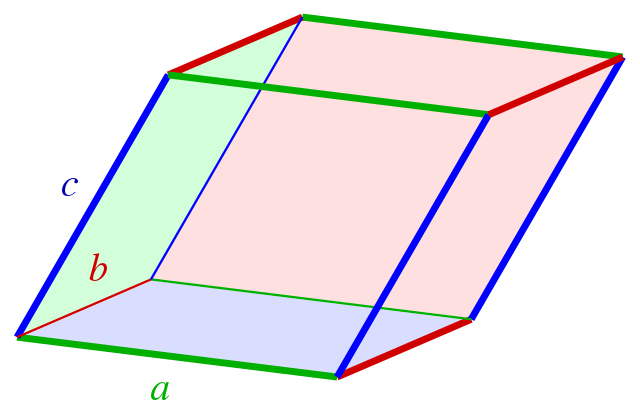
\includegraphics[width=0.6 \textwidth]{images/640px-Parallelepiped-0}    
\end{figure}
Es gilt  $$  \text{vol} \bigr( P(a_1, \cdots, a_n) \bigr) =  | det (a_1, \cdots, a_n) |   \; .$$

\href{https://www.math.uchicago.edu/~may/VIGRE/VIGRE2007/REUPapers/FINALAPP/Peng.pdf}{Ausfürlicher Beweis}

\end{proof}


\begin{Definition}[Diffeomorphismus]
Seien $U$ und $V$ offene Teilmengen des $\mathbb{R}^n$. Eine Abbildung  $T: U \to V$ heißt diffeomorphismus, wenn eine  Umkehrfunktion $T^{-1}: V  \to U$ existiert, also $T^{-1} (T (u)) = u$ gilt für alle $u \in U$, die ebenfalls differenzierbar ist.
\end{Definition}

\begin{Beispiel}
Für eine invertiertere Matrix $A$ ist $T(x):= Ax$ ein Diffeomorphismus.
\end{Beispiel}

\begin{Satz}
Seien $U$ und $V$ offene Teilmengen des $\mathbb{R}^n$, $T: U \to V$ ein Diffeomorpismus und $f: V \to \mathbb{R}$ eine integrierbare Funktion. Dann gilt:
$$ \int_V  f(y)  d \mu = \int_U f(T (x))  \cdot | \det(T' (x)) | d \mu   \; .$$
\end{Satz}
\begin{proof}
Seien $I_k \in \mathbb{I}(n)$ Quader, $J_k := T(I_k)$ und $b_k = T(c_k)$. Dann ist 
$$\sum_{k=1}^n  b_k  \text{vol}(J_k) \approx  \sum_{k=1}^n T(c_k) \cdot | \det T' (c_k)|  \text{vol}(I_k) \; .$$
Die Behauptung folgt dann (nicht trivial) durch den Übergang zu Grenzwerten mit entsprechenden Konvergenzsätzen.
\end{proof}




\subsubsection{Parameterabhängige Integrale}

\begin{Definition}
Eine Folge von Funktionen $f_k$ konvergiert Punktweise fast überall gegen eine Funktion $f$, falls es eine Nullmenge $N$ gibt, mit 
$\lim_{k \to \infty} f_k (x) = f(x)$ für alle $x \in \mathbb{R}^n \setminus N$.
\end{Definition}

\begin{Satz}[Satz von Lebesgue]
Sei $f_k$ eine Folge integrierbarer Funktionen auf $\mathbb{R}^n$ die fast überall Punktweise gegen eine Funktion $f$ konvergiert.
Es gebe eine integrierbare Funktion $F$ mit $|f_k (x)| \leq F(x) $ für alle $x \in \mathbb{R}^n$ und alles $k$. Dann ist $f$ integrierbar und es gilt
$$ \int f(x) d \mu = \lim_{k \to \infty} f_k(x) d \mu $$
\end{Satz}

Sei $f: X \times T \subset \mathbb{R}^{n-p} \times \mathbb{R}^p$ eine Funktion, so dass für festes $x \in X$ die Funktion $f_x(t) := f(x,t)$ über $T$ integrierbar ist. Durch Integration erhält man die Funktion 
$$ F(x) := \int_T f(x,t)  d \mu_T$$ 
auf $X$.

\begin{Satz}[Stetigkeitssatz]
$f$ habe zusätzlich die Eigenschaften:
\begin{itemize}
\item Für festes $t$ ist $f_t(x):= f(x,z)$ stetig.
\item Es gibt auf $T$ eine integrierbare Funktion $\phi$ mit $\phi(t) \geq 0$ und $|f(x,t)| \leq \phi(t)$ für alle $(x,t) \in X \times T$.
\end{itemize}
Dann ist die oben definierte Funktion $F$ stetig. 
\end{Satz}
\begin{proof}
Sei  $x_k \to x$   eine konvergente Folge in $X$ und $f_k(t):= f(x_k,t)$. Nach Voraussetzung konvergiert diese Folge Punktweise gegen die Funktion $f_x(t)$ und $| f_k (x) | \leq \phi(x)$. Mit dem Satz von Lebesgue folgt
$$ \lim_{k \to \infty} \int_T f_k(t) d \mu_T = \int_T f(x,t) d \mu_T$$
und damit $ \lim_{k \to \infty} F(x_k) =  F(x)$.
\end{proof}

\begin{Satz}[Differentiationssatz]
$f$ habe zusätzlich die Eigenschaften:
\begin{itemize}
\item Für festes $t$ ist $f_t(x):= f(x,t)$ stetig differenzierbar.
\item Es gibt auf $T$ eine integrierbare Funktion $\phi$ mit $\phi(t) \geq 0$ und $| \frac{\partial}{\partial x_i} f(x,t)| \leq \phi(t)$ für alle $(x,t) \in X \times T$ und $i=1, \cdots n-p$.
\end{itemize}
Dann ist die oben definierte Funktion $F$ stetig differenzierbar und es gilt
$$\frac{\partial}{\partial x_k} F(x)  = \int_T \frac{\partial}{\partial x_k} f(x,t) d \mu_T \; .$$ 
\end{Satz}
\begin{proof}
Sei $x_k := x_0 + h_k e_i$ und 
$$ \varphi_k (t) := \frac{f(x_k,t)  - f(x_0,t)  }{h_k} \; .$$
Damit sind die Funktionen  $\varphi_k $ integrierbar und für jedes $t \in T$ gilt

$$  \lim_{k \to \infty} \varphi_k (t) = \frac{\partial}{\partial x_i}f(x_0, t) \; .$$
Mit dem Satz von Lebesgue gilt
$$ \lim_{k \to \infty}  \int_T \varphi_k (t) d \mu_T = \int_T   \frac{\partial}{\partial x_i}f(x_0, t) d \mu_T $$
und da 
$$  \int_T \varphi_k (t) d \mu_T = \frac{F(x_k) -F(x_0)}{h_k}$$ ist, folgt die Behauptung.
 
\end{proof}




\subsubsection{Faltung}
\begin{Definition}
Für integrierbare Funktionen  $f$ und $g$ auf $\mathbb{R}^n$ ist die Faltung definiert durch
\begin{align}
(f * g )(x) := \int_{\mathbb{R}^n}  f(x- y) \cdot g(y) \; d \mu_y  \; .
\end{align}
Das Integral existiert wegen dem Satz von Fubini.  Nach Anwendung der Transformation $y \to x -y$  ist  
\begin{align}
(f * g )(x) := \int_{\mathbb{R}^n}  f(y) \cdot g(x-y) \; d \mu_y  \; .
\end{align}
und damit $f*g = g*f$
\end{Definition}


\begin{Satz}
Für die Faltung gilt
\begin{itemize}
\item $ \int (f * g) d \mu = \int f d \mu \cdot \int g d \mu$.
\item $||f *g ||_1 \leq ||f||_1 \cdot ||g||_1$.
\end{itemize}
\end{Satz}
\begin{proof}
Die erste Behauptung folgt durch Vertauschen der Integrationsreihenfolge (möglich wegen Fubini) und Anwendung des Produktsatzes.
Die Zweite aus $| f*g| \leq |f| \cdot |g|$.
\end{proof}


\begin{Satz}[Differentiationssatz der Faltung]
Für die Faltung gilt bei entsprechenden Voraussetzungen der Differenzierbarkeit der Funktionen 
$$ \partial^{\alpha} (f  * g) = f * \partial^{\alpha} g \; .$$
\end{Satz}
\begin{proof}
Nach Anwendung der Transformation $y \to x -y$ folgt die Aussage direkt aus dem Differentiationssatz.
\end{proof}

\begin{Definition}
Eine Folge von messbaren Funktionen $\delta_k : \mathbb{R}^n \to \mathbb{R}$ heißt Dirac-Folge, falls gilt:
\begin{itemize}
\item $\delta_k (x) \geq 0$ für alle $x \in \mathbb {R}^n$ und alle $k$.
\item $\int_{\mathbb{R}^n} \delta_k d \mu = 1$ für alle $k$.
\item Für jede Kugel $B_r(0)$ ist $\lim_{k \to \infty} \int_{\mathbb{R}^n \setminus B_r(0)} \delta_k = 0$
\end{itemize}
\end{Definition}


\begin{Beispiel}[Variable Glockenkurve]
\label{Diracfolgeb}
Definiere $\delta_1 (t) := \frac{1}{(2 \pi)^{\frac{n}{2}}} e^{ \frac{ - || t ||^2}{2}}$ und $\delta_k(t) := k^n \delta_1(k t)$.  
Für das Integral erhalten wir $\int_{\mathbb{R}^n} \delta_1 (t)  d \mu_n = 1$. Um dies einzusehen betrachten wir den Spezialfall
\begin{align*}
& I := \int_{0}^{\infty} e^{-x^2} \; dx\\
& I^2 = \int_{0}^{\infty} \int_{0}^{\infty} e^{-(x^2+y^2)} \; dx \;dy \\
&x=r \cos \varphi ,y=r\sin \varphi ,r^2 = x^2 + y^2  \; (\text{ da } \cos^2 + \sin^2 = 1)\\
 &\text{ \href{https://de.wikipedia.org/wiki/Polarkoordinaten\#Zylinderkoordinaten}{LINK: Polarkoordinatentransformation}} \\
& = \int_{0}^{\frac{\pi}{2}}  \int_{0}^{\infty}r \cdot e^{-r^2} \; dr \;d\varphi \\
&= \frac{\pi}{2} \int_{0}^{\infty}r \cdot e^{-r^2} \; dr \\
&= -\frac{\pi}{4} [e^{-r^2} ]_0^{\infty} = \frac{\pi}{4} \Rightarrow I = \frac{\sqrt{\pi}}{2}
\end{align*}
Mit der skalierung $T(t) : = \frac{t}{k}$ folgt mit dem Transformationssatz $\int \delta_k (t) d \mu = \int  k^n \delta_1(k t) d \mu = 1$.
\end{Beispiel}

\begin{Satz}[Approximationssatz]
Für eine Integrierbare Funktion $f$ und eine Dirac-Folge $\delta$ gilt $|| f -  f *\delta_k ||_1 \to 0 $. Die Folge  $f *\delta_k$ konvergiert also in der $L^1$-Norm gegen $f$.
\end{Satz}
\begin{figure}[H]
      \centering
    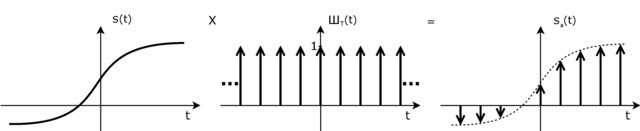
\includegraphics[width=0.9\textwidth]{images/640px-Dirac-comb_-_Sampling}
\caption{Quelle: Wikipedia: https://commons.wikimedia.org/wiki/File:Dirac-comb\_-\_Sampling.png}
\end{figure}



\subsubsection{Fouriertransformation}
Eine Funktion $g :\mathbb{R}^n \to \mathbb{C}$ heißt integrierbar, wenn sowohl ihr Realteil $\text{Re}(g) $ als auch ihr Imaginärteil $\text{Im}(g) $  integrierbar sind. In diesem Fall setzen wir
$$ \int_{\mathbb{R}^n} g d \mu :=  \int_{\mathbb{R}^n}  \text{Re}(g) d \mu  + i \int_{\mathbb{R}^n}  \text{Im}(g) d \mu$$
\begin{Definition}
Sei $f: \mathbb{R}^n \to \mathbb{R}$ eine integrierbare Funktion. Ihre Fouriertransformierte ist definiert durch 
$$ \hat{f}(x) :=  \frac{1}{ (2 \pi)^{\frac{n}{2}}} \int_{\mathbb{R}^n} f  \cdot e^{ - i \langle x , t  \rangle }d \mu_{t}  $$
\end{Definition}

Aufgrund der Linearität des Integrals und da $\int f^2 d \mu  \geq 0$ wegen $f^2(x) \geq 0$ gilt, können wir das Integral als Skalarpdukt (hermetische Produkt)
$$ \langle f ,g \rangle_{L^1} := \int f \cdot g d \mu$$
auf dem Raum der integrierbaren Funktion betrachten.  Mit $ e^{i z} = \cos(z) + i\cdot  \sin(z) $ können wir die Fouriertransformierte am Punkt $x$ als den Anteil  der  Frequenz $x$ innerhalb des Signals interpretieren. 

\begin{Beispiel}
\label{hatgleichf}
Für $f(t) := e^{- \frac{ ||t||^2 }{2}}$ gilt $\hat{f} = f$.
\end{Beispiel}
\begin{proof}
\href{https://mathworld.wolfram.com/FourierTransformGaussian.html}{Beweis für $n=1$}.
Für $n > 1$ erhalten wir mit der Produktdarstellung $e^{- \frac{ ||t||^2 }{2}} \cdot e^{ - i \langle x , t  \rangle } = \prod_{k=1}^n e^{-\frac{t_k^2}{2}} \cdot e^{-ix_kt_k}$ und dem Produktsatz
\begin{align*}
\hat{f}(x)  =  \prod_{k=1}^n \frac{1}{\sqrt{2 \pi}} \int_{\mathbb{R} } e^{-\frac{t_k^2}{2}} \cdot e^{-ix_kt_k} d \mu_t = \prod_{k=1}^n e^{-i \frac{x^2_k}{2}} = f(x)
\end{align*}

\end{proof}

\begin{Satz}[Umkehrsatz]
Sei $f :\mathbb{R}^n \to \mathbb{R}$ eine integrierbare Funktion. Dann gilt überall bis auf einer Nullmenge
\begin{align}
\label{Spektraldarstellung}
f(t) =  \frac{1}{ (2 \pi)^{\frac{n}{2}}}  \int_{\mathbb{R}^n} \hat{f}(x)  \cdot e^{i \langle x , t  \rangle } d \mu_{x}   \; .
\end{align}
Kurz $\hat{\hat{f}}(t) = f(-t)$. Gleichheit gilt an jedem Punkt, an dem $f$ stetig ist.
Gleichung \ref{Spektraldarstellung} wird auch die Spektraldarstellung von $f$ genannt.
\end{Satz}
\begin{proof}
Für die  Dirac-Folge $\delta_k$ aus Beispiel \ref{Diracfolgeb} ist nach Beispiel \ref{hatgleichf}  $\hat{\delta_1} = \delta_1$  und damit
\begin{align*}
\delta_k(t) =   \frac{k^n}{(2 \pi)^n} \int_{\mathbb{R}^n} e^{- \frac{|| \xi ||^2}{2}}  \cdot e^{i \langle \xi , k t  \rangle }  d \mu_{\xi}  
= \frac{1}{(2 \pi)^n} \int_{\mathbb{R}^n} e^{- \frac{|| x ||^2}{2k^2}}  \cdot e^{i \langle x ,  t  \rangle }  d \mu_{x}  \;.
\end{align*}

Falten mit  $f$ ergibt 
\begin{align*}
(f * \delta_k)(t) = \frac{1}{(2 \pi)^n} \int_{\mathbb{R}^n}\int_{\mathbb{R}^n} f(s) e^{- \frac{|| x ||^2}{2k^2}}  \cdot e^{i \langle x ,  t - s  \rangle }  d \mu_{x}   d \mu_s
\end{align*}
Vertauschen der Integrationsreihenfolge und auswerten des inneren Integrals ergibt 

\begin{align*}
(f * \delta_k)(t) = \frac{1}{(2 \pi)^n} \int_{\mathbb{R}^n}  \hat{f}(x)  e^{i \langle x ,  t  \rangle }  e^{- \frac{|| x ||^2}{2k^2}}  d \mu_{x}  \; .
\end{align*}
Für $k \to \infty$ konvergiert der Integrant $ \hat{f}(x) e^{i \langle x ,  t  \rangle }  e^{- \frac{|| x ||^2}{2k^2}} \to \hat{f}(x) e^{i \langle x ,  t  \rangle } $. Nach dem Satz von Lebesgue konvergiert die Folge $(f *\delta_k)(t)$ gegen $ \frac{1}{(2 \pi)^n} \int_{\mathbb{R}^n}  \hat{f}(x)  e^{i \langle x ,  t  \rangle } d \mu_{x} $. Andererseits konvergiert die Folge $(f *\delta_k)(t)$ nach dem Approximationssatz gegen $f$.
\end{proof}
 
\begin{Satz}[Shannon-Abtasttheorem]
Eine stetige, integrierbare Funktion $f: \mathbb{R} \to \mathbb{R}$, dessen Fouriertransformierte $\hat{f}$ eines Intervall $(-b,b) \subset \mathbb{R}$ verschwindet, kann für jedes $T$ mit $T < \frac{pi}{b}$ aus Ihren Funktionswerten $f(kT)$ mit $k \in \mathbb{Z}$ rekonstruiert werden. Insbesondere gilt
$$ f(x) = \sum_{k= -\infty}^{\infty} f(kT) \cdot \text{sinc} \biggl (   \frac{\pi}{T}(x - k T) \biggr)$$  mit 
$ \text{sinc}(x):=  \frac{\sin(x)}{x}$.
\end{Satz}
\begin{proof}
Da $\hat{f}$ stetig und beschränkt ist, ist $\hat{f}$ integrierbar und nach dem Umkehrsatz gilt
$$ f(x) = \frac{1}{\sqrt{2 \pi}} \int_{\frac{- \pi}{T}}^{\frac{ \pi}{T}} \hat{f}(\xi) e^{ix \xi} \; .$$
Es seien $F(\xi):= \hat{f}(\xi)$ und $G_x(\xi):=\frac{1}{\sqrt{2 \pi}} e^{-ix \xi}$. Ihre Fourierkoeffizienten sind gegeben durch
\begin{align*}
\hat{F}(k) = \sqrt{\frac{T}{2 \pi}} \int_{\frac{- \pi}{T}}^{\frac{ \pi}{T}} \hat{f} (\xi) e^{ikT \xi}  d \xi = \sqrt{T} f(kT)  \\
\hat{G}(k) =  \frac{\sqrt{T}}{2 \pi} \int_{\frac{- \pi}{T}}^{\frac{ \pi}{T}}  e^{-i (x-kT) \xi}  d \xi = \frac{1}{\sqrt{T} }  \text{sinc} \biggl (   \frac{\pi}{T}(x - k T) \biggr)
\end{align*}
Nach der Parsevalschen Formel gilt
\begin{align*}
f(x) =  \int_{\frac{- \pi}{T}}^{\frac{- \pi}{T}} F(\xi) \overline{G_x(\xi)} d \xi =  \sum_{k= -\infty}^{\infty} \hat{F}(k) \overline {\hat{G}_x (k) } \; . 
\end{align*}
 
\end{proof}

\subsubsection{Diskrete Fouriertransformation}

%Mit dem Umkehrsatz gilt
%$$f(t)= \frac{1}{\sqrt{2 \pi}} \int_{-\infty}^\infty \hat f(\omega) e^{i \omega t} \, \mathrm d \omega
%$$
Im eindimensionalen Fall ist die Fouriertransformation einer Funktion gegeben durch
$$
\hat f(\omega)= \frac{1}{\sqrt{2 \pi}} \int_{-\infty}^\infty f(t) e^{-i \omega t} \, \mathrm d t.
$$
Wählen wir einen Radius $R$ so groß, dass außerhalb des Intervalls $[-R,R]$ nur noch ein unwesentlicher Teil von $f$ liegt, ist $f$ außerdem stetig und eine Zahl $N$ so groß gewählt, dass $T:=R/N$ klein genug ist, um $f$ sinnvoll singulär,  durch Funktionswerte $f(kT)$, abzutasten, so kann das Fourierintegral in der Transformationsformel sinnvoll durch eine Summe ersetzt werden:
$$
\hat f(\omega)\approx F(\omega)=\frac{1}{\sqrt{2 \pi}} \sum_{k=-N}^N e^{-i \omega kT}f(kT) \,T \;.
$$

Die diskrete Fouriertransformation (DFT) eines diskreten Signals $(a_0, \cdots a_{N-1})$ ist dann definiert durch vielfaches
$\hat{a_i} : = \sum_{j=0}^{N-1} e^{-2 \pi i \frac{jk}{N}} a_j$. 
Für höhere Dimensionen diskretisiert man analog in alle Koordinatenrichtungen. 

%Das entspricht, bis auf einen konstanten Faktor $T/\sqrt{2 \pi}$ der Berechnungsformel der DFT. Der Vektor $x=( f(-NT),\dotsc,f(NT))$ hat 
%$2N+1$ Elemente. Wir wissen bereits, dass es ausreicht, die Frequenzkoeffizienten für die$2N+1$ Frequenzen $\omega_n:=2\pi\cdot \frac{n}{(2N+1)T}$mit $n=-N,\dotsc,-1,0,1,\dotsc,N$ zu bestimmen, um die Funktionswerte im Vektor $x$ zu rekonstruieren. Mit der notwendigen Anpassung der Konstanten in der iDFT erhalten wir
%$$
%(nT)=\frac{1}{\sqrt{2 \pi}}\sum_{k=-N}^N e^{i \omega_k nT}F(\omega_k)\,\frac{2\pi}{(2N+1)T}.
%$$
%Der Diskretisierungsabstand im Frequenzbereich ist proportional zu $1/R$, also nach Voraussetzung ebenfalls klein, sodass diese Berechnung der Diskretisierung der inversen Fourier-Transformation entspricht.
